\documentclass[aspectratio=169,10pt]{beamer}

% =========================================================
% PACKAGES
% =========================================================
\usepackage[T1]{fontenc}
\usepackage[utf8]{inputenc}
\usepackage[default]{sourcesanspro}
\usepackage{graphicx}
\usepackage{tikz}
\usetikzlibrary{positioning,arrows.meta,calc}
\usepackage{xcolor}
\usepackage{ragged2e}
\usepackage{hyperref}

% =========================================================
% PORTFOLIO COLOURS
% =========================================================
\definecolor{PortfolioTeal}{HTML}{007977}
\definecolor{PortfolioOrange}{HTML}{F28C28}
\definecolor{PortfolioBlue}{HTML}{3B82C4}
\definecolor{SoftTeal}{HTML}{E8F3F2}
\definecolor{SoftBlue}{HTML}{EEF5FA}
\definecolor{SoftOrange}{HTML}{FBECDD}
\definecolor{SoftGrey}{HTML}{F2F4F5}
\definecolor{TextGrey}{HTML}{3B4145}
\definecolor{LineGrey}{HTML}{CBD2D6}

\setbeamercolor{normal text}{fg=TextGrey,bg=white}
\setbeamercolor{frametitle}{fg=white,bg=PortfolioTeal}
\setbeamercolor{structure}{fg=PortfolioTeal}
\setbeamercolor{itemize item}{fg=PortfolioTeal}
\setbeamercolor{itemize subitem}{fg=PortfolioTeal}

\setbeamertemplate{navigation symbols}{}
\setbeamertemplate{itemize item}
{\raise0.12ex\hbox{\scriptsize$\blacktriangleright$}}
\setbeamertemplate{itemize subitem}
{\raise0.10ex\hbox{\tiny$\blacktriangleright$}}

\setbeamerfont{frametitle}{
	size=\Large,
	series=\mdseries
}

\setbeamerfont{title}{
	size=\fontsize{25}{29}\selectfont,
	series=\mdseries
}

\setbeamerfont{subtitle}{
	size=\large,
	series=\mdseries
}

% =========================================================
% HEADER / FOOTER
% =========================================================
\setbeamertemplate{frametitle}{%
	\nointerlineskip
	\begin{beamercolorbox}[
		wd=\paperwidth,
		ht=0.82cm,
		dp=0.20cm,
		leftskip=0.42cm
		]{frametitle}
		\usebeamerfont{frametitle}
		\insertframetitle
	\end{beamercolorbox}%
}

\setbeamertemplate{footline}{%
	\leavevmode%
	\hbox{%
		\begin{beamercolorbox}[
			wd=.82\paperwidth,
			ht=0.34cm,
			dp=0.11cm,
			leftskip=0.35cm
			]{author in head/foot}%
			\color{TextGrey}\scriptsize
			Valentin Ochioiu
			\hspace{0.13cm}|\hspace{0.13cm}
			Network Security Portfolio
		\end{beamercolorbox}%
		\begin{beamercolorbox}[
			wd=.18\paperwidth,
			ht=0.34cm,
			dp=0.11cm,
			rightskip=0.35cm plus1fil
			]{date in head/foot}%
			\color{TextGrey}\scriptsize
			\hfill
			\insertframenumber\ / \inserttotalframenumber
		\end{beamercolorbox}%
	}%
}

% =========================================================
% REUSABLE ELEMENTS
% =========================================================
\newcommand{\boxtext}[4][SoftGrey]{%
	\begingroup
	\setlength{\fboxsep}{7pt}%
	\colorbox{#1}{%
		\parbox{\dimexpr\linewidth-2\fboxsep\relax}{%
\RaggedRight
			{\color{#2}\large #3}
			\par
			\vspace{0.07cm}
			{\small #4}%
		}%
	}%
	\endgroup
}

\newcommand{\compactbox}[4][SoftGrey]{%
	\begingroup
	\setlength{\fboxsep}{6pt}%
	\colorbox{#1}{%
		\parbox{\dimexpr\linewidth-2\fboxsep\relax}{%
\RaggedRight
			{\color{#2}\normalsize #3}
			\par
			\vspace{0.04cm}
			{\scriptsize #4}%
		}%
	}%
	\endgroup
}

\newcommand{\smallnote}[1]{%
	\par
	\vspace{0.05cm}
	{\scriptsize\color{TextGrey}#1\par}
}

\newcommand{\sectionlabel}[1]{%
	{\color{PortfolioTeal}\large #1}
}

\newcommand{\bluelabel}[1]{%
	{\color{PortfolioBlue}\large #1}
}

\newcommand{\orangelabel}[1]{%
	{\color{PortfolioOrange}\large #1}
}

\graphicspath{{images/}}

% =========================================================
% DOCUMENT INFO
% =========================================================
\title{Windows AppLocker \& Group Policy Security Lab}

\subtitle{
	Application Control with Path, Publisher and File Hash Rules
}

\author{Valentin Ochioiu}

\institute{
	Folkuniversitetet, Gothenburg
}

\date{5 February 2026}

\begin{document}
	
	% =========================================================
	% 1. TITLE
	% =========================================================
	{
		\setbeamercolor{background canvas}{bg=PortfolioTeal}
		\setbeamertemplate{footline}{}
		
		\begin{frame}[plain]
			
			\begin{tikzpicture}[remember picture,overlay]
				
				\fill[PortfolioTeal]
				(current page.south west)
				rectangle
				(current page.north east);
				
				\draw[
				PortfolioOrange,
				line width=2.2pt
				]
				([xshift=0.75cm,yshift=-5.55cm]
				current page.north west)
				--
				([xshift=-0.75cm,yshift=-5.55cm]
				current page.north east);
				
			\end{tikzpicture}
			
			\vspace{1.15cm}
			
			{\color{white}
				\usebeamerfont{title}
				\inserttitle
				\par
			}
			
			\vspace{0.20cm}
			
			{\color{white!88}
				\usebeamerfont{subtitle}
				\insertsubtitle
				\par
			}
			
			\vfill
\vspace*{1.15cm}
			
			\begin{columns}[T,onlytextwidth]
				
				\column{0.50\textwidth}
				
				{\color{white}\large Valentin Ochioiu}
				\par
				
				{\color{white!82}\small
					Network Security Student
				}
				
				\column{0.50\textwidth}
				
				\raggedleft
				
				{\color{white}\large
					Folkuniversitetet, Gothenburg
				}
				\par
				
				{\color{white!82}\small
					5 February 2026
				}
				
			\end{columns}
			
			\vspace{-0.70cm}
			
		\end{frame}
	}
	
	% =========================================================
	% 2. PROJECT OVERVIEW
	% =========================================================
	\begin{frame}{Project Overview}
		
		\begin{columns}[T,onlytextwidth]
			
			\column{0.60\textwidth}
			
			{\large
				Windows application control using AppLocker policy
			}
			\par
			
			\vspace{0.12cm}
			
			\small
			
			The lab focused on controlling which applications a Windows
			user could execute. AppLocker was tested with several rule
			conditions instead of one broad allow-list.
			
			\vspace{0.22cm}
			
			\sectionlabel{Implemented}
			
			\begin{itemize}
				\small
				\setlength\itemsep{0.06cm}
				
				\item Default Windows and administrator rules
				
				\item User-specific path-based Deny rule for Notepad++
				
				\item Restrictive allow-listing with file-hash rules
				
				\item Publisher, Path and Hash conditions in one policy
				
				\item Windows Installer, Script and Packaged App
				rule collections
				
				\item Functional testing and AppLocker
				event-log verification
				
			\end{itemize}
			
			\column{0.36\textwidth}
			
			\boxtext[SoftTeal]
			{PortfolioTeal}
			{Core security idea}
			{
				Only applications matching approved rules should execute.
				Rule scope can depend on identity, path, publisher signature
				or exact file identity.
			}
			
			\vspace{0.17cm}
			
			\boxtext[SoftOrange]
			{PortfolioOrange}
			{Scope}
			{
				This presentation covers only the Windows AppLocker and
				Group Policy work from the lab, using local rules and standard-user execution tests.
			}
			
		\end{columns}
		
	\end{frame}
	
	% =========================================================
	% 3. TEST MODEL
	% =========================================================
	\begin{frame}{Test Model}
		
		\begin{columns}[T,onlytextwidth]
			
			\column{0.45\textwidth}
			
			\compactbox[SoftBlue]
			{PortfolioBlue}
			{Windows test system}
			{
				Windows Server 2022 was the AppLocker test host.
				Rules were configured through Local Group Policy,
				with Application Identity enabled for enforcement.
			}
			
			\vspace{0.14cm}
			
			\compactbox[SoftTeal]
			{PortfolioTeal}
			{Identity model}
			{
				Administrator access was preserved.
				A dedicated \textbf{TestUser} was used to validate
				restrictions from a standard-user perspective.
			}
			
			\vspace{0.14cm}
			
			\compactbox[SoftGrey]
			{PortfolioTeal}
			{Test cycle}
			{
				Windows host: 192.168.122.20. After policy changes, run \texttt{gpupdate /force}, launch applications as TestUser and inspect AppLocker events.
			}
			
			\column{0.51\textwidth}
			
			\sectionlabel{How the policy was tested}
			
			\vspace{0.10cm}
			
			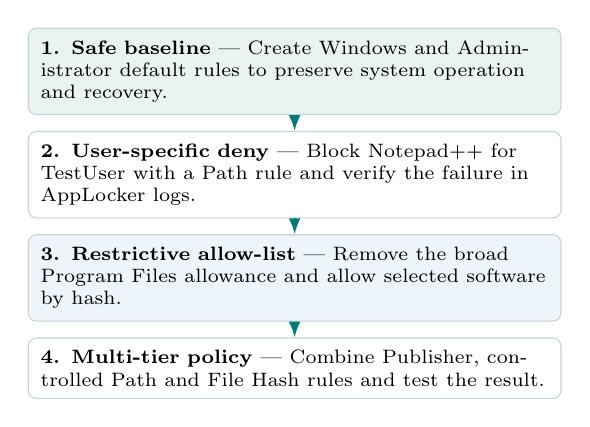
\begin{tikzpicture}[
				node distance=0.20cm,
				stepbox/.style={
					draw=LineGrey,
					rounded corners=3pt,
					fill=white,
					text width=6.45cm,
					minimum height=0.72cm,
					align=left,
					inner sep=4.5pt,
					font=\scriptsize
				},
				arr/.style={
					-{Latex[length=2mm]},
					draw=PortfolioTeal,
					thick
				}
				]
				
				\node[
				stepbox,
				fill=SoftTeal
				] (s1) {
					\textbf{1. Safe baseline} —
					Create Windows and Administrator default rules
					to preserve system operation and recovery.
				};
				
				\node[
				stepbox,
				below=of s1
				] (s2) {
					\textbf{2. User-specific deny} —
					Block Notepad++ for TestUser with a Path rule
					and verify the failure in AppLocker logs.
				};
				
				\node[
				stepbox,
				below=of s2,
				fill=SoftBlue
				] (s3) {
					\textbf{3. Restrictive allow-list} —
					Remove the broad Program Files allowance
					and allow selected software by hash.
				};
				
				\node[
				stepbox,
				below=of s3
				] (s4) {
					\textbf{4. Multi-tier policy} —
					Combine Publisher, controlled Path and File Hash
					rules and test the result.
				};
				
				\draw[arr] (s1) -- (s2);
				\draw[arr] (s2) -- (s3);
				\draw[arr] (s3) -- (s4);
				
			\end{tikzpicture}
			
		\end{columns}
		
	\end{frame}
	
	% =========================================================
	% 4. CONFIGURATION
	% =========================================================
	\begin{frame}{AppLocker Configuration and Enforcement}
		
		\begin{columns}[T,onlytextwidth]
			
			\column{0.49\textwidth}
			
			\centering
			
			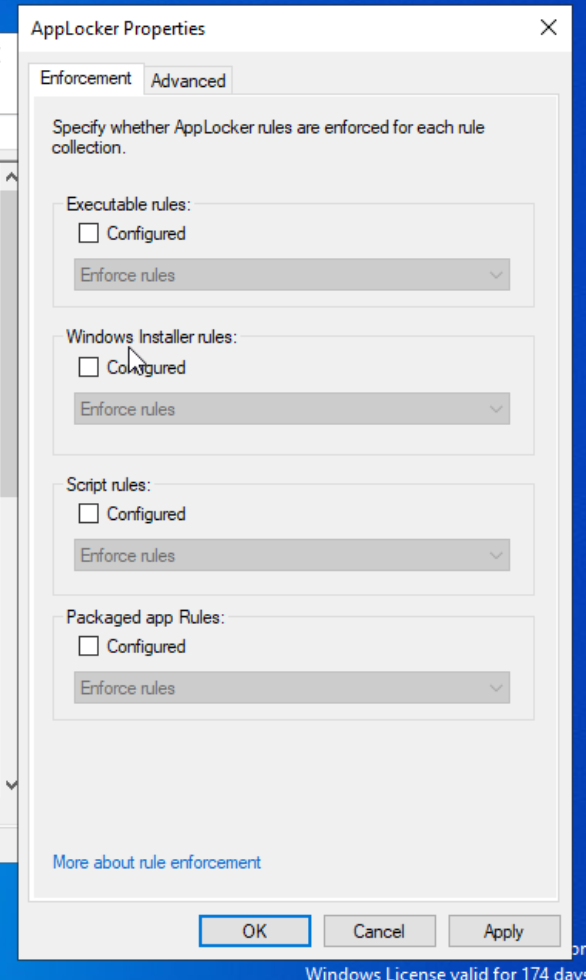
\includegraphics[
			width=\linewidth,
			height=4.65cm,
			keepaspectratio
			]{applocker.png}
			
			\smallnote{
				Initial configuration view, before selecting collection enforcement.
			}
			
			\column{0.47\textwidth}
			
			\centering
			
			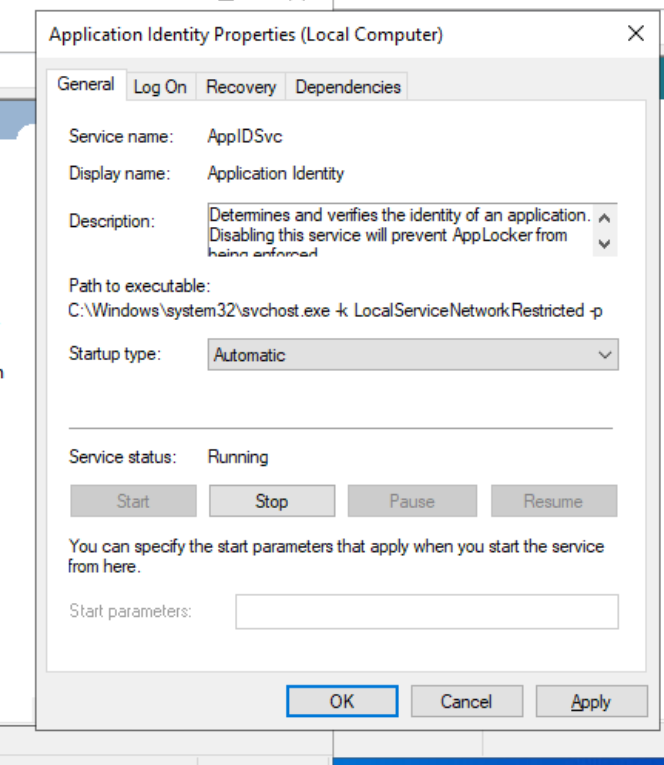
\includegraphics[
			width=\linewidth,
			height=3.65cm,
			keepaspectratio
			]{application-identity-service.png}
			
			\smallnote{
				Application Identity service properties used during testing.
			}
			
			\vspace{0.14cm}
			
			\boxtext[SoftTeal]
			{PortfolioTeal}
			{Implemented}
			{
				Application Identity is running. Later execution tests and block events demonstrate enforcement. The setup capture at left still shows unselected configuration boxes.
			}
			
		\end{columns}
		
	\end{frame}
	
	% =========================================================
	% 5. DEFAULT RULES
	% =========================================================
	\begin{frame}{Default Rules and an Important Failure Case}
		
		\begin{columns}[T,onlytextwidth]
			
			\column{0.52\textwidth}
			
			\centering
			
			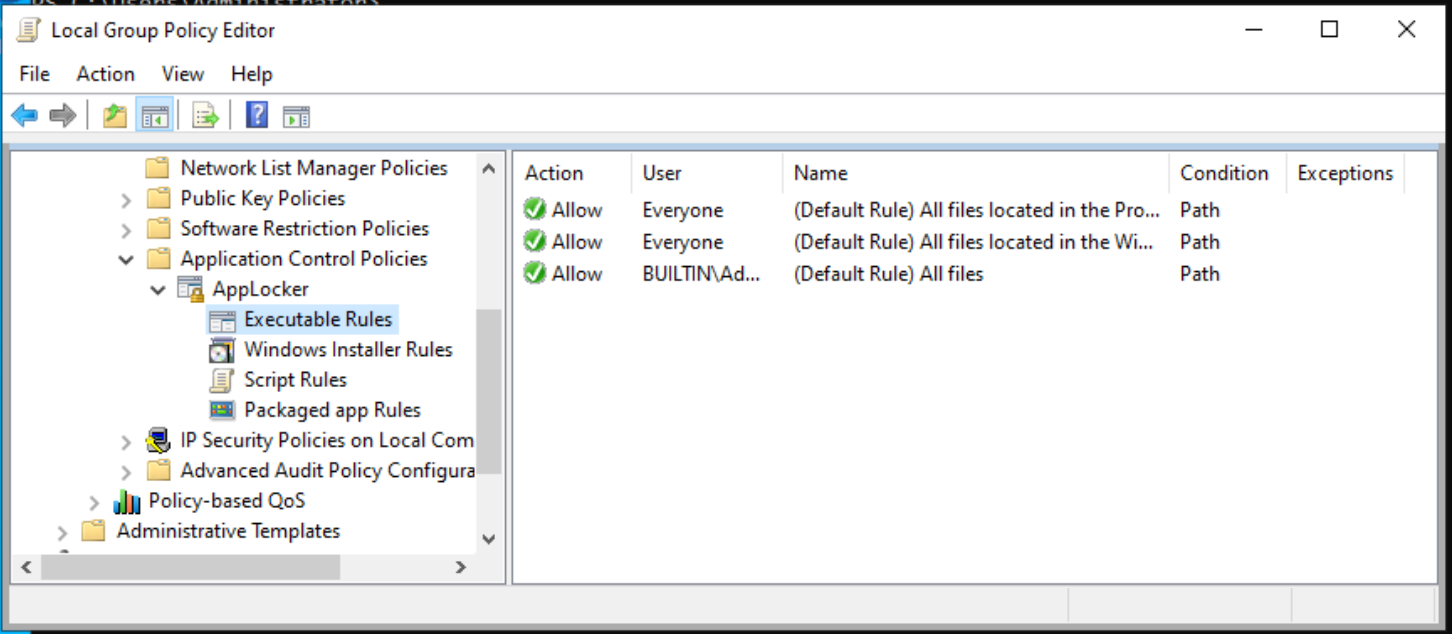
\includegraphics[
			width=\linewidth,
			height=3.25cm,
			keepaspectratio
			]{defaul-rules-for-all.png}
			
			\smallnote{
				Default executable rules retained for Windows
				and administrators.
			}
			
			\vspace{0.12cm}
			
			\boxtext[SoftTeal]
			{PortfolioTeal}
			{Why they mattered}
			{
				The Windows-folder rule preserved essential system execution,
				while the administrator rule kept full administrative access
				during testing.
			}
			
			\column{0.44\textwidth}
			
			\boxtext[SoftOrange]
			{PortfolioOrange}
			{Failure case}
			{
				Removing the Windows default rule blocked important
				system files. The shell failed to start and recovery
				required Safe Mode and disabling AppLocker.
			}
			
			\vspace{0.18cm}
			
			\sectionlabel{Lesson learned}
			
			\begin{itemize}
				\small
				\setlength\itemsep{0.08cm}
				
				\item Default-deny can affect the operating system itself.
				
				\item Trusted system execution must be preserved explicitly.
				
				\item Restrictive policies should be introduced incrementally.
				
			\end{itemize}
			
		\end{columns}
		
	\end{frame}
	
	% =========================================================
	% 6. PATH RULE
	% =========================================================
	\begin{frame}{User-Specific Path Rule — Notepad++}
		
		\begin{columns}[T,onlytextwidth]
			
			\column{0.52\textwidth}
			
			\centering
			
			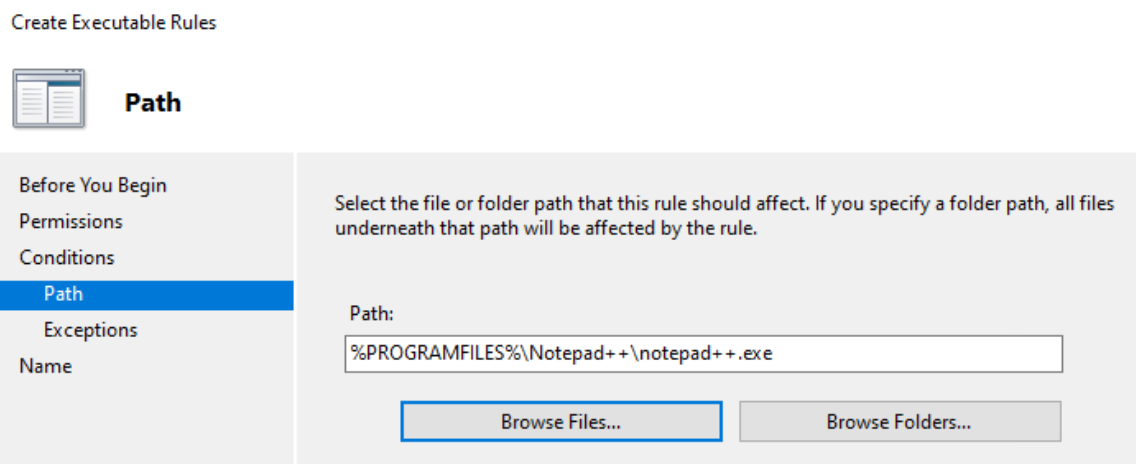
\includegraphics[
			width=\linewidth,
			height=4.05cm,
			keepaspectratio
			]{path-rule-for-notepad.png}
			
			\smallnote{
				Path condition configured for the Notepad++ executable.
			}
			
			\column{0.44\textwidth}
			
			\sectionlabel{Policy objective}
			
			\small
			
			Block Notepad++ for one user rather than for every account
			on the system.
			
			\vspace{0.13cm}
			
			\begin{itemize}
				\small
				\setlength\itemsep{0.08cm}
				
				\item Created a dedicated \textbf{TestUser}.
				
				\item Added a path-based \textbf{Deny} rule.
				
				\item Scoped the rule to TestUser.
				
				\item Retained the Windows defaults for stability.
				
			\end{itemize}
			
			\vspace{0.14cm}
			
			\boxtext[SoftBlue]
			{PortfolioBlue}
			{Security value}
			{
				AppLocker can enforce different application rights
				for different user identities on the same Windows system.
			}
			
		\end{columns}
		
	\end{frame}
	
	% =========================================================
	% 7. PATH VALIDATION
	% =========================================================
	\begin{frame}{Path Rule Validation — Blocked Execution}
		
		\begin{columns}[T,onlytextwidth]
			
			\column{0.54\textwidth}
			
			\centering
			
			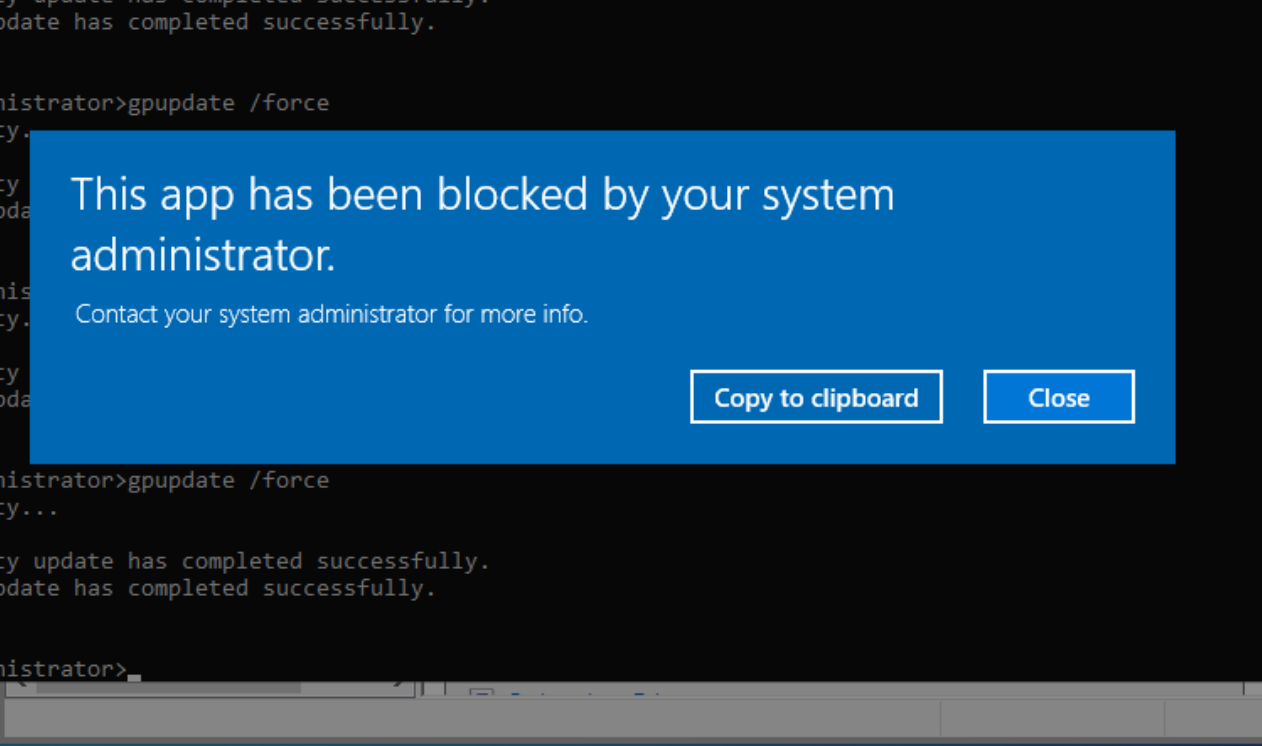
\includegraphics[
			width=\linewidth,
			height=4.35cm,
			keepaspectratio
			]{finally-applocker-blocks.png}
			
			\smallnote{
				Observed result: the application was blocked by system policy.
			}
			
			\column{0.42\textwidth}
			
			\centering
			
			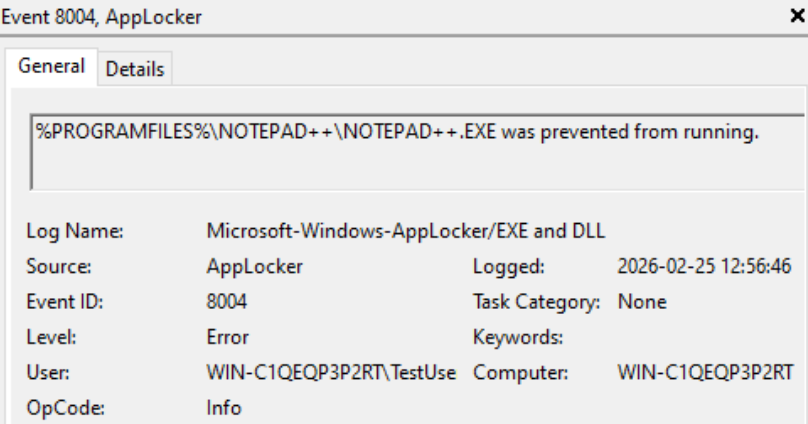
\includegraphics[
			width=\linewidth,
			height=2.45cm,
			keepaspectratio
			]{blocked-notepad.png}
			
			\smallnote{
				AppLocker event recording the prevented execution.
			}
			
			\vspace{0.13cm}
			
			\boxtext[SoftTeal]
			{PortfolioTeal}
			{Validated}
			{
				The application was actually prevented from running
				and the AppLocker log recorded the enforcement event.
			}
			
		\end{columns}
		
	\end{frame}
	
	% =========================================================
	% 8. HASH MODEL
	% =========================================================
	\begin{frame}{Hash-Based Rule Under a More Restrictive Policy}
		
		\begin{columns}[T,onlytextwidth]
			
			\column{0.53\textwidth}
			
			\centering
			
			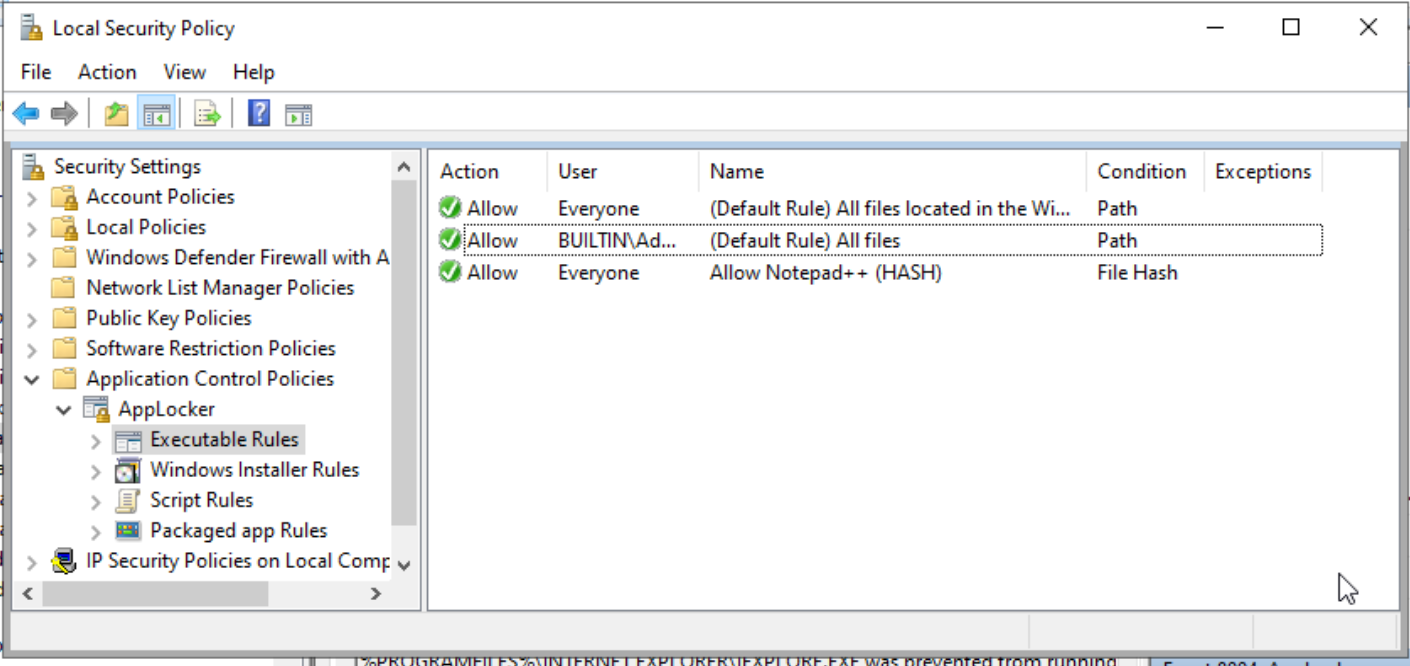
\includegraphics[
			width=\linewidth,
			height=3.55cm,
			keepaspectratio
			]{hash-rule-for-notepad.png}
			
			\smallnote{
				Executable rules after removing the broad
				Program Files allowance.
			}
			
			\column{0.43\textwidth}
			
			\sectionlabel{Policy change}
			
			\begin{itemize}
				\small
				\setlength\itemsep{0.08cm}
				
				\item Administrator access to all files was retained.
				
				\item The broad
				\textit{Allow Everyone — Program Files}
				rule was removed.
				
				\item A hash rule allowed one specifically approved executable.
				
				\item The Windows rule remained for system stability.
				
			\end{itemize}
			
			\vspace{0.13cm}
			
			\boxtext[SoftOrange]
			{PortfolioOrange}
			{Default-deny effect}
			{
				Once the broad Program Files allow rule was removed,
				software without another matching Allow rule was
				blocked automatically.
			}
			
		\end{columns}
		
	\end{frame}
	
	% =========================================================
	% 9. HASH VALIDATION
	% =========================================================
	\begin{frame}{Hash Rule Validation and Default-Deny Behaviour}
		
		\begin{columns}[T,onlytextwidth]
			
			\column{0.52\textwidth}
			
			\centering
			
			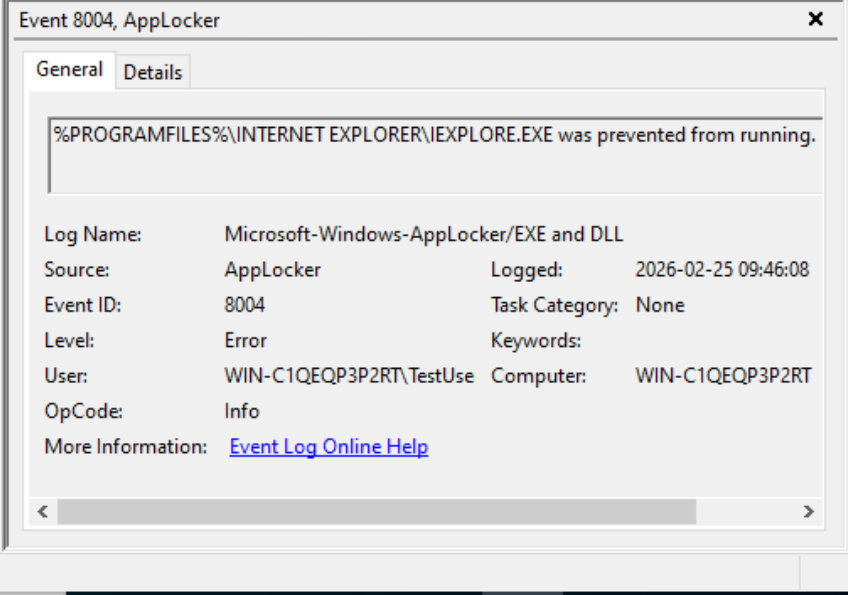
\includegraphics[
			width=\linewidth,
			height=4.25cm,
			keepaspectratio
			]{event-viewer-explorer-blocked.png}
			
			\smallnote{
				AppLocker Event Viewer evidence from the restrictive-rule test.
			}
			
			\column{0.44\textwidth}
			
			\centering
			
			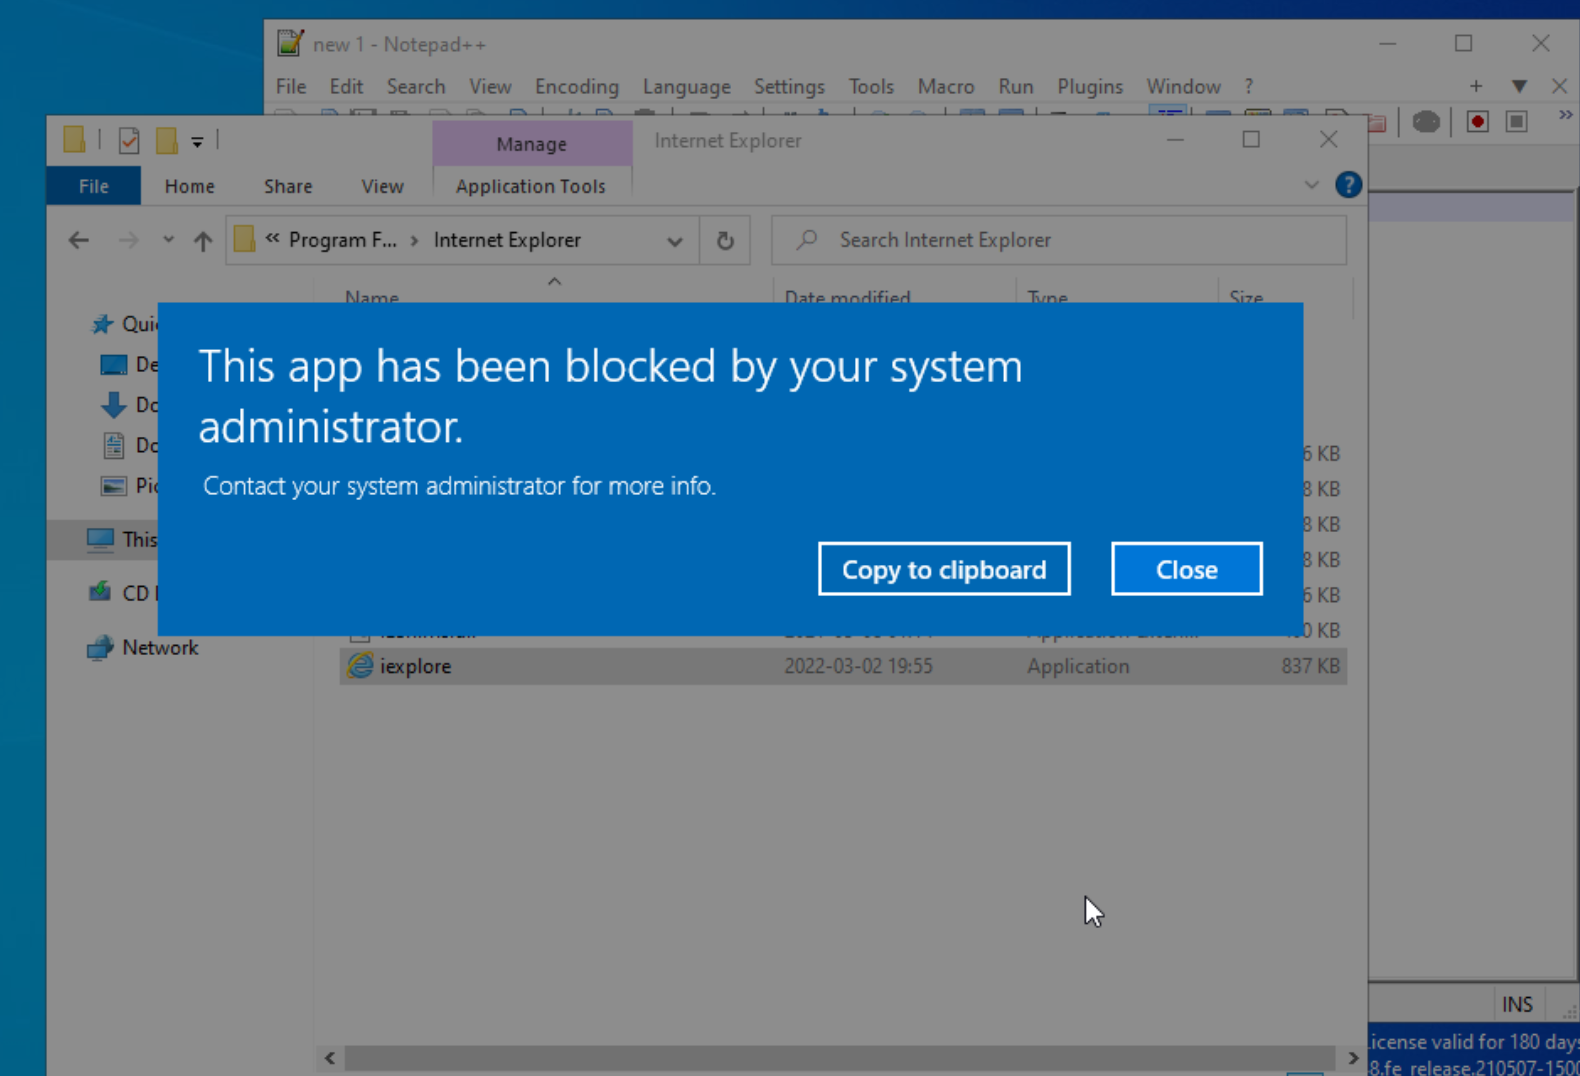
\includegraphics[
			width=\linewidth,
			height=2.45cm,
			keepaspectratio
			]{notepad-works-with-hash-but-everything-else-blocked.png}
			
			\smallnote{
				Internet Explorer shown as one blocked example.
			}
			
			\vspace{0.13cm}
			
			\boxtext[SoftBlue]
			{PortfolioBlue}
			{Observed behaviour}
			{
				Internet Explorer was not special-cased.
				It was simply one visible example of expected
				default-deny behaviour: after the broad Program Files
				Allow rule was removed, other Program Files applications
				were also blocked unless another Allow rule matched.
			}
			
		\end{columns}
		
	\end{frame}
	
	% =========================================================
	% 10. MULTI-TIER POLICY
	% =========================================================
	\begin{frame}{Multi-Tier Application Control Policy}
		
		\begin{columns}[T,onlytextwidth]
			
			\column{0.60\textwidth}
			
			\centering
			
			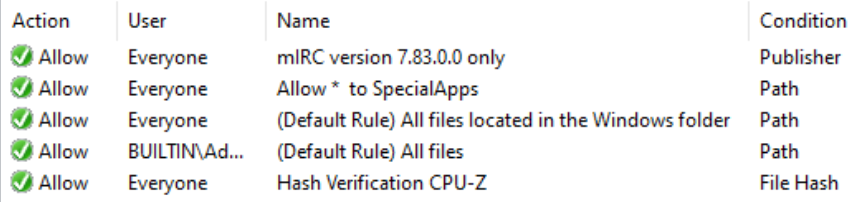
\includegraphics[
			width=\linewidth,
			height=4.80cm,
			keepaspectratio
			]{screenshot-from-2026-02-26-14-27-07.png}
			
			\smallnote{
				Combined executable rule set using multiple
				AppLocker condition types.
			}
			
			\column{0.36\textwidth}
			
			\boxtext[SoftTeal]
			{PortfolioTeal}
			{Publisher}
			{
				Allowed signed mIRC using publisher and version criteria.
			}
			
			\vspace{0.13cm}
			
			\boxtext[SoftBlue]
			{PortfolioBlue}
			{Path}
			{
				Allowed programs stored in the designated
				SpecialApps directory.
			}
			
			\vspace{0.13cm}
			
			\boxtext[SoftOrange]
			{PortfolioOrange}
			{File hash}
			{
				Allowed one exact CPU-Z executable by file identity.
			}
			
		\end{columns}
		
	\end{frame}
	
	% =========================================================
	% 11. PUBLISHER RULE
	% =========================================================
	\begin{frame}{Publisher Rule — Signed Application Control}
		
		\begin{columns}[T,onlytextwidth]
			
			\column{0.57\textwidth}
			
			\centering
			
			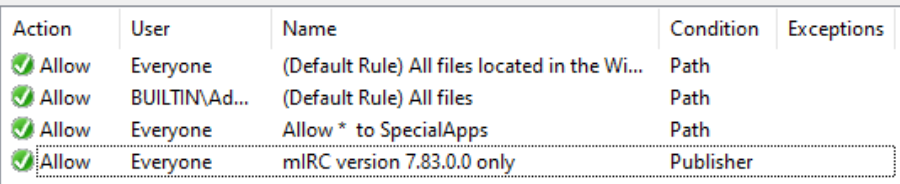
\includegraphics[
			width=\linewidth,
			height=4.15cm,
			keepaspectratio
			]{publisher-allow-on-specific-version-rule.png}
			
			\smallnote{
				Executable policy including the mIRC Publisher rule.
			}
			
			\column{0.39\textwidth}
			
			\sectionlabel{Implemented}
			
			\begin{itemize}
				\small
				\setlength\itemsep{0.08cm}
				
				\item Publisher condition referencing mIRC version 7.83.0.0.
				
				\item Trust based on digital-signature identity
				rather than only file location.
				
			\end{itemize}
			
			\vspace{0.15cm}
			
			\boxtext[SoftBlue]
			{PortfolioBlue}
			{Why use it?}
			{
				Publisher rules are useful for signed software when policy
				should follow publisher, product or version information.
			}
			
		\end{columns}
		
	\end{frame}
	
	% =========================================================
	% 12. PATH ALLOW
	% =========================================================
	\begin{frame}{Path Rule — Controlled SpecialApps Directory}
		
		\begin{columns}[T,onlytextwidth]
			
			\column{0.58\textwidth}
			
			\centering
			
			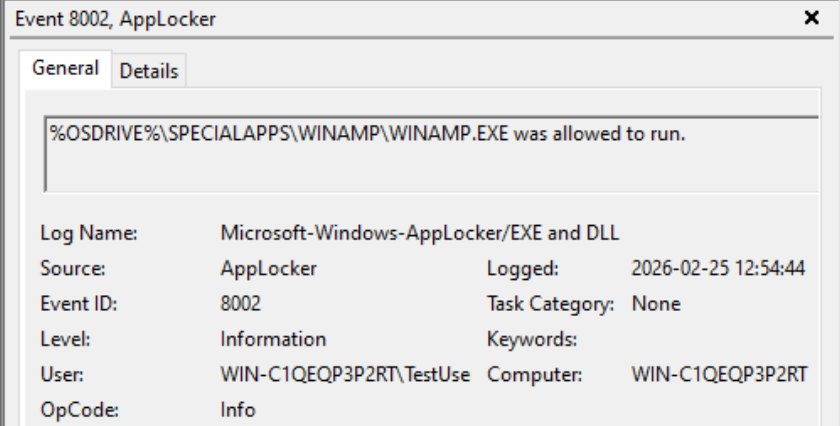
\includegraphics[
			width=\linewidth,
			height=4.70cm,
			keepaspectratio
			]{winamp-allowed-to-run-on-testuser.png}
			
			\smallnote{
				Event 8002: Winamp in SpecialApps was allowed for TestUser.
			}
			
			\column{0.38\textwidth}
			
			\sectionlabel{Implemented rule}
			
			\small
			
			Programs stored under the designated
			\textbf{SpecialApps} path were allowed.
			Software outside approved conditions remained
			subject to default-deny.
			
			\vspace{0.17cm}
			
			\boxtext[SoftOrange]
			{PortfolioOrange}
			{Security consideration}
			{
				A path rule is only as trustworthy as the permissions
				protecting that directory. A user-writable allowed path
				can become a route for unapproved software.
			}
			
		\end{columns}
		
	\end{frame}
	
	% =========================================================
	% 13. CPU-Z HASH RULE
	% =========================================================
	\begin{frame}{File Hash Rule -- CPU-Z Evidence}

\includegraphics[width=.85\textwidth,height=.55cm,keepaspectratio]{cpuz-rule-row.png}
\smallnote{The policy identifies ``Hash Verification CPU-Z'' with condition File Hash.}
\vspace{.16cm}
\begin{columns}[T,onlytextwidth]
\column{.48\textwidth}
\sectionlabel{Allowed execution: Event 8002}\par\vspace{.08cm}
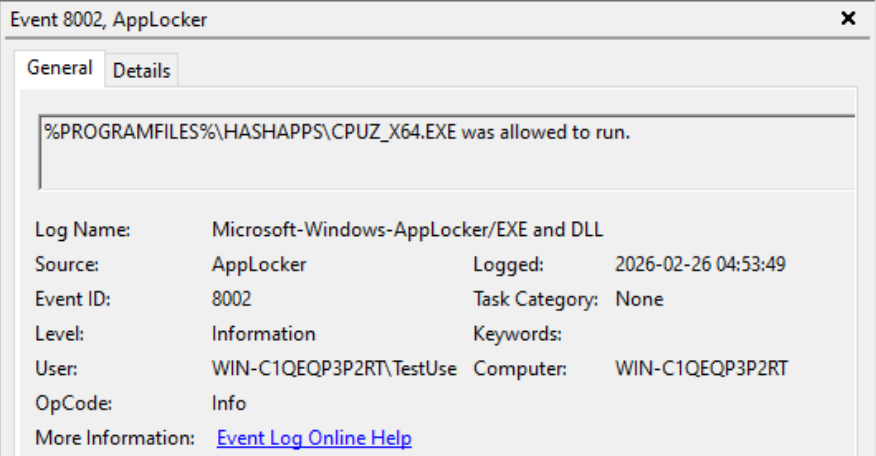
\includegraphics[width=\linewidth,height=2.95cm,keepaspectratio]{hashrule-approved.png}
\column{.48\textwidth}
\sectionlabel{Blocked execution: Event 8004}\par\vspace{.08cm}
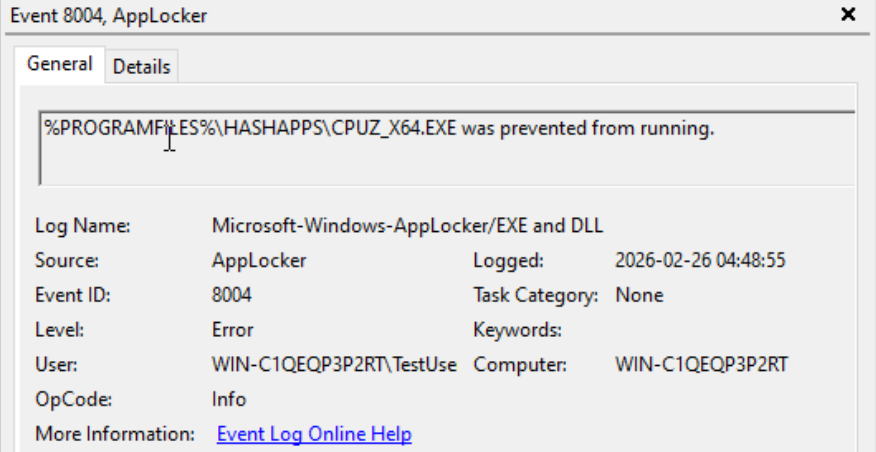
\includegraphics[width=\linewidth,height=2.95cm,keepaspectratio]{cpuz-blocked.png}
\end{columns}
\vspace{.14cm}
\compactbox[SoftOrange]{PortfolioOrange}{Hash value is not visible in the lab captures}
{The ZIP shows the File Hash rule and CPU-Z execution events, but no hash-condition dialog or raw value. The events alone do not establish what changed between tests. AppLocker uses an Authenticode hash to identify the approved file.}
\end{frame}
	
	% =========================================================
	% 14. OTHER RULE COLLECTIONS
	% =========================================================
	\begin{frame}{Windows Installer, Script and Packaged App Rules}
\begin{columns}[T,onlytextwidth]
\column{.73\textwidth}
\sectionlabel{Windows Installer}\par\vspace{.06cm}
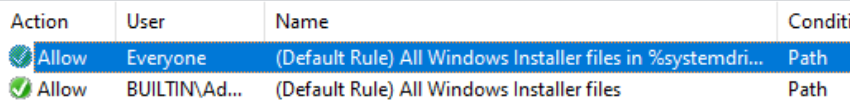
\includegraphics[width=\linewidth]{windows-installer-rules.png}
\smallnote{Windows Installer folder allowance and administrator default.}
\vspace{.22cm}
\sectionlabel{Script}\par\vspace{.06cm}
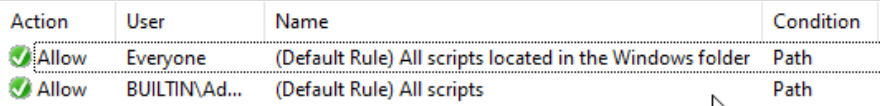
\includegraphics[width=\linewidth]{script-rules.png}
\smallnote{Windows-folder scripts and administrator default.}
\vspace{.22cm}
\sectionlabel{Packaged App}\par\vspace{.06cm}
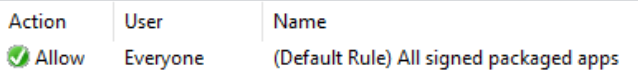
\includegraphics[width=.9\linewidth]{packaged-apps.png}
\smallnote{The captured default allows all signed packaged apps.}
\column{.23\textwidth}
\compactbox[SoftTeal]{PortfolioTeal}{Collection scope}
{Each collection has its own rules. Executable rules alone do not define script, installer or packaged-app permissions.}
\vspace{.18cm}
\compactbox[SoftOrange]{PortfolioOrange}{Lab evidence}
{The signed packaged-app default is a broad allowance. This capture does not demonstrate a restricted app-by-app policy.}
\end{columns}
\end{frame}
	
	% =========================================================
	% 15. LIMITATIONS / BYPASS SURFACE
	% =========================================================
	\begin{frame}{AppLocker Limitations and Bypass Surface}
\orangelabel{Production context -- not implemented or tested in this lab}
\vspace{.25cm}
\begin{itemize}\small\setlength\itemsep{.24cm}
\item \textbf{DLL side-loading:} the DLL collection is disabled by default. Without it, executable allow rules do not check the DLLs an approved application loads.
\item \textbf{Trusted binaries (LOLBins):} allowed signed system tools can provide proxy execution paths. A trusted signature alone does not make every use safe.
\item \textbf{Writable paths:} users who can write to an allowed folder may place unapproved software there. Directory permissions are part of the trust decision.
\item \textbf{Coverage gaps:} some interpreted content and host processes fall outside direct AppLocker checks. Complement application rules with endpoint monitoring and least privilege.
\end{itemize}
\vspace{.18cm}
{\scriptsize Microsoft Learn: \href{https://learn.microsoft.com/en-us/windows/security/application-security/application-control/app-control-for-business/applocker/working-with-applocker-rules}{Working with AppLocker rules}; \href{https://learn.microsoft.com/en-us/windows/security/application-security/application-control/app-control-for-business/applocker/security-considerations-for-applocker}{Security considerations for AppLocker}.}
\end{frame}
	
	% =========================================================
	% 16. TROUBLESHOOTING
	% =========================================================
	\begin{frame}{Troubleshooting and Lessons Learned}
		
		\begin{columns}[T,onlytextwidth]
			
			\column{0.31\textwidth}
			
			\boxtext[SoftOrange]
			{PortfolioOrange}
			{1. System stability}
			{
				Removing essential Windows allowances blocked core
				processes and broke the shell. Safe Mode recovery
				was required.
			}
			
			\column{0.31\textwidth}
			
			\boxtext[SoftBlue]
			{PortfolioBlue}
			{2. Rule precision}
			{
				Path, Publisher and Hash conditions solve different
				application-control problems and have different
				maintenance trade-offs.
			}
			
			\column{0.31\textwidth}
			
			\boxtext[SoftTeal]
			{PortfolioTeal}
			{3. Validation}
			{
				Execution tests and AppLocker event logs were used
				to confirm that policy changes were actually enforced.
			}
			
		\end{columns}
		
		\vspace{0.28cm}
		
		\boxtext[SoftGrey]
		{PortfolioTeal}
		{Practical takeaway}
		{
			Introduce allow-listing changes incrementally, test them
			with non-administrative users, preserve a recovery path,
			and verify the result in AppLocker logs before broader
			enforcement.
		}
		
	\end{frame}
	
	% =========================================================
	% 17. PRODUCTION CONSIDERATIONS
	% =========================================================
	\begin{frame}{Production Security Considerations}
		
		\begin{columns}[T,onlytextwidth]
			
			\column{0.47\textwidth}
			
			\sectionlabel{Lab approach}
			
			\begin{itemize}
				\small
				\setlength\itemsep{0.07cm}
				
				\item Windows Server 2022 test system
				
				\item Local Group Policy configuration
				
				\item TestUser for enforcement validation
				
				\item Default-deny behaviour
				
				\item Publisher, Path and File Hash conditions
				
				\item Manual functional and event-log verification
				
			\end{itemize}
			
			\column{0.49\textwidth}
			
			\bluelabel{Production improvements to consider}
			
			\begin{itemize}
				\small
				\setlength\itemsep{0.07cm}
				
				\item Stage new policies in Audit only mode first
				
				\item Deploy centrally through domain Group Policy or MDM
				
				\item Scope policies by OU and security group
				
				\item Monitor AppLocker events centrally
				
				\item Prefer maintainable signed-software rules
				where practical
				
				\item Review writable paths, exceptions and trusted
				system binaries
				
			\end{itemize}
			
		\end{columns}
		
		\vspace{0.18cm}
		
		\boxtext[SoftOrange]
		{PortfolioOrange}
		{Important distinction}
		{
			These are production recommendations identified after
			the exercise. Central domain deployment, audit-mode staging
			and the stronger controls discussed here are not claimed
			as features implemented in the original lab.
		}
		
	\end{frame}
	
	% =========================================================
	% 18. SUMMARY
	% =========================================================
	\begin{frame}{Project Summary}
		
		\begin{columns}[T,onlytextwidth]
			
			\column{0.49\textwidth}
			
			\sectionlabel{Implemented}
			
			\begin{itemize}
				\small
				\setlength\itemsep{0.07cm}
				
				\item AppLocker enforcement through local Group Policy
				
				\item Default Windows and administrator rules
				
				\item User-specific path-based Deny rule
				
				\item Restrictive File Hash allow-listing
				
				\item Publisher, Path and Hash multi-tier policy
				
				\item Installer, Script and Packaged App collections
				
			\end{itemize}
			
			\vspace{0.12cm}
			
			\bluelabel{Validated}
			
			\begin{itemize}
				\small
				\setlength\itemsep{0.07cm}
				
				\item Blocked execution for TestUser
				
				\item Expected default-deny behaviour
				
				\item AppLocker Event Viewer evidence
				
				\item Recovery from an over-restrictive policy
				
			\end{itemize}
			
			\column{0.47\textwidth}
			
			\boxtext[SoftBlue]
			{PortfolioBlue}
			{Result}
			{
				The lab demonstrated practical Windows application
				control with several AppLocker rule types and a progressively
				more restrictive policy model.
				
				\par
				\vspace{0.12cm}
				
				The strongest lesson was not simply how to create a rule,
				but how to balance application trust, user scope,
				system stability, validation, maintenance and recovery.
			}
			
		\end{columns}
		
	\end{frame}
	
\end{document}